\documentclass{beamer}
\mode<presentation> {
%\usetheme{Madrid}
%\usetheme{default}
\usepackage{color}
\definecolor{bottomcolour}{rgb}{0.21,0.11,0.21}
\definecolor{middlecolour}{rgb}{0.21,0.11,0.21}
\setbeamercolor{structure}{fg=white}
\setbeamertemplate{frametitle}[default]%[center]
\setbeamercolor{normal text}{bg=black, fg=white}
\setbeamertemplate{background canvas}[vertical shading]
[bottom=bottomcolour, middle=middlecolour, top=black]
\setbeamertemplate{items}[circle]
\setbeamertemplate{navigation symbols}{} %no nav symbols
\setbeamercolor{block title}{use=structure,fg=white,bg=structure.fg!50!red!50!blue!100!green}
\setbeamercolor{block body}{parent=normal text,use=block title,bg=block title.bg!5!white!10!bg,fg=white}
\setbeamertemplate{navigation symbols}{}
}

\usepackage{graphicx} 
\usepackage{booktabs} 
\usepackage[utf8]{inputenc}  
\usepackage[T1]{fontenc}  
\usepackage{geometry}     
\usepackage[francais]{babel} 
\usepackage{eurosym}
\usepackage{verbatim}
\usepackage{ragged2e}
\justifying

%%%%%%%%%%%%%%%%%%%%%%%%%%%%%%%%%%%%%%%%%%%%%%%%%%%%%%%%%%%%%%%%
%% ccBeamer 0.1, 2007-07-02                                   %%
%% Written by Sebastian Pipping <webmaster@hartwork.org>      %%
%% ---------------------------------------------------------- %%
%% Licensed under Creative Commons Attribution-ShareAlike 3.0 %%
%% http://creativecommons.org/licenses/by-sa/3.0/             %%
%%%%%%%%%%%%%%%%%%%%%%%%%%%%%%%%%%%%%%%%%%%%%%%%%%%%%%%%%%%%%%%%


%% Images
\newcommand{\CcImageBy}[1]{%
	
\includegraphics[scale=#1]{creative_commons/cc_by_30.pdf}%
}
\newcommand{\CcImageCc}[1]{%
	
\includegraphics[scale=#1]{creative_commons/cc_cc_30.pdf}%
}
\newcommand{\CcImageDevNations}[1]{%
	
\includegraphics[scale=#1]{creative_commons/cc_dev_nations_30.pdf}%
}
\newcommand{\CcImageNc}[1]{%
	
\includegraphics[scale=#1]{creative_commons/cc_nc_30.pdf}%
}
\newcommand{\CcImageNd}[1]{%
	
\includegraphics[scale=#1]{creative_commons/cc_nd_30.pdf}%
}
\newcommand{\CcImagePd}[1]{%
	
\includegraphics[scale=#1]{creative_commons/cc_pd_30.pdf}%
}
\newcommand{\CcImageSa}[1]{%
	
\includegraphics[scale=#1]{creative_commons/cc_sa_30.pdf}%
}
\newcommand{\CcImageSampling}[1]{%
	
\includegraphics[scale=#1]{creative_commons/cc_sampling_30.pdf}%
}
\newcommand{\CcImageSamplingPlus}[1]{%
	
\includegraphics[scale=#1]{creative_commons/cc_sampling_plus_30.pdf}%
}


%% Groups
\newcommand{\CcGroupBy}[1]{% zoom
	\CcImageBy{#1}%
}
\newcommand{\CcGroupByNc}[2]{% zoom, gap
	\CcImageBy{#1}\hspace*{#2}\CcImageNc{#1}%
}
\newcommand{\CcGroupByNcNd}[2]{% zoom, gap
	\CcImageBy{#1}\hspace*{#2}\CcImageNc{#1}\hspace*{#2}\CcImageNd{#1}%
}
\newcommand{\CcGroupByNcSa}[2]{% zoom, gap
	\CcImageBy{#1}\hspace*{#2}\CcImageNc{#1}\hspace*{#2}\CcImageSa{#1}%
}
\newcommand{\CcGroupByNd}[2]{% zoom, gap
	\CcImageBy{#1}\hspace*{#2}\CcImageNd{#1}%
}
\newcommand{\CcGroupBySa}[2]{% zoom, gap
	\CcImageBy{#1}\hspace*{#2}\CcImageSa{#1}%
}
\newcommand{\CcGroupDevNations}[1]{% zoom
	\CcImageDevNations{#1}%
}
\newcommand{\CcGroupNcSampling}[2]{% zoom, gap
	\CcImageNc{#1}\hspace*{#2}\CcImageSampling{#1}%
}
\newcommand{\CcGroupPd}[1]{% zoom
	\CcImagePd{#1}%
}
\newcommand{\CcGroupSampling}[1]{% zoom
	\CcImageSampling{#1}%
}
\newcommand{\CcGroupSamplingPlus}[1]{% zoom
	\CcImageSamplingPlus{#1}%
}


%% Text
\newcommand{\CcLongnameBy}{Attribution}
\newcommand{\CcLongnameByNc}{Attribution-NonCommercial}
\newcommand{\CcLongnameByNcNd}{Attribution-NoDerivs}
\newcommand{\CcLongnameByNcSa}{Attribution-NonCommercial-ShareAlike}
\newcommand{\CcLongnameByNd}{Attribution-NoDerivs}
\newcommand{\CcLongnameBySa}{Attribution-ShareAlike}

\newcommand{\CcNote}[1]{% longname
	This work is licensed under the \textit{Creative Commons #1 3.0 License}.%
}


\title[Les Chiffrofêtes]{Des cryptoparty au Café vie privée \\Le chiffrement est en pleine démocratisation} 
\author{Genma}

\begin{document}

%% Titlepage
\begin{frame}
	\begin{center}
	 	\huge{Des cryptoparty au Café vie privée, \\le chiffrement est en pleine démocratisation}
	 	\\
		\Large{Genma}
	 	\\~\\
		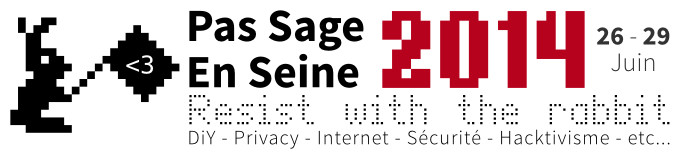
\includegraphics[scale=0.5] {logoPSES.jpg} 
		\\~\\
		\CcGroupByNcSa{0.83}{0.95ex}\\
		{\tiny\CcNote{\CcLongnameByNcSa}}
		\vspace*{-2.5ex}
	\end{center}
\end{frame}



%----------------------------------------------------------------------------------------

\begin{frame}
\frametitle{
\includegraphics[scale=0.4]{./Genma.jpg} \ \ \  A propos de moi  }
\begin{columns}[c] 

\column{.55\textwidth} 
\textbf{Où me trouver sur Internet?}
\begin{itemize}
\item Le Blog de Genma : http://genma.free.fr
\item Twitter : http://twitter.com/genma
\end{itemize}

\textbf{Mes centres d'intérêts?}
\\ Plein de choses dont:
\begin{itemize}
\item La veille technologique
\item Le chiffrement
\end{itemize}

\column{.5\textwidth} 
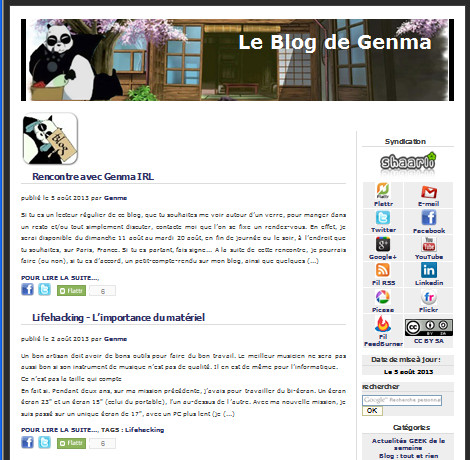
\includegraphics[width=5cm,height=5cm]{./blog.jpg} 

\end{columns}
\end{frame}

%----------------------------------------------------------------------------------------
\begin{frame}
\begin{center}
\Huge{Les Chiffrofêtes }
\end{center}
\end{frame}

%------------------------------------------------
\begin{frame}
\frametitle{Qu'est ce qu'une chiffrofête?}

\begin{block}{Chiffrofête, cryptopartie...}
\begin{itemize}
\justifying{
\item Le terme de cryptoparty (contraction de crypto - chiffrement et party - partie, fête) est souvent francisé en cryptopartie mais nous utilisons le terme de chiffrofête (contraction de chiffrement et fête) qui se veut une traduction moins connoté de ce terme.

\begin{itemize}
\justifying{
\item Connoté au sens où cryptoparty est très lié au monde des hackerspaces, underground...
}
\end{itemize}

\item L'autre appellation que nous utilisons pour ce même type d'évènement est les Cafés vie privée.
}
\end{itemize}
\end{block}
\end{frame}

%------------------------------------------------
\begin{frame}
\frametitle{Quand cela a-t-il commencé?}

\begin{itemize}
\justifying{ 
\item Les cryptoparty existent depuis longtemps. Mais c'est en octobre 2013, à l'intiative, entre autre d'Amaelle Guiton et d'Okhin qu'a été lancé le premier Café vie privée.
\item Et c'est en novembre 2013, lors de l'Ubuntu Party et des ateliers Prism Break qu'Okhin a appelé ça des chiffrofêtes.
}
\end{itemize}
Depuis, au moins un évènement au lieu tous les mois.
\end{frame}



%------------------------------------------------
\begin{frame}
\frametitle{Le public concerné}

\begin{block}{Quel est le public ciblé/concerné par les chiffrofêtes?}
Le public est cible des chiffrofêtes est divers et varié :
\begin{itemize}
\justifying{
\item Les journalistes et autres professions à risques ;
\item  Ls scolaires (Lycéens, étudiants) ;
\item Les geeks, libristes et autres technophiles ;
\item  Mais surtout Grand public (tout âge confondu).
}
\end{itemize}
\justifying{
D'une façon générale, ce peut être toute personne sensibilisée / concernée par les problématiques de la vie privée, de la sécurisation de ses communications...
}
\end{block}
\end{frame}

%----------------------------------------------------------------------------------------
\begin{frame}
\begin{center}
\Huge{Comment ça se passe?}
\end{center}
\end{frame}


%------------------------------------------------
\begin{frame}
\frametitle{Le concept des chiffrofêtes}

\justifying{
Il suffit d'un lieu où se réunir, d'animateurs désirant partager leurs connaissances et d'un public désireux d'en savoir plus, qui a envie d'apprendre.
}

\end{frame}

%------------------------------------------------
\begin{frame}
\frametitle{Ateliers, conférences, débats}

\justifying{
Au début, on fait une rapide présentation des sujets qui peuvent être abordés. Ensuite, des groupes se forment et se déroulent alors : 
\begin{itemize}
\item  une mini-conférence/un talk de présentation ;
\item  un atelier (chacun installe et manipule sur ma machine) ;
\item  un débat/scéance de questions réponses.
\end{itemize}
La durée idéale est d'une heure et demi. Avec deux scéances, on remplit un après-midi.
}
\end{frame}

%------------------------------------------------
\begin{frame}
\frametitle{Les logiciels 1/2}

\begin{block}{Le logiciel libre}
\justifying{
Les outils présentés sont donc tous compatibles Linux, Windows et Mac et/ou y possèdent des alternatives, et on parle aussi des problèmes rencontrés sur mobile.
\begin{itemize}
\item Dès que possible, c'est le logiciel libre qui est privilégié. Chacun vient avec son ordinateur et quelque soit le système d'exploitation (GNU\/Linux, MacOSX, Windows, Android), les logiciels les plus adaptés sont proposés, installés.
\item Mais Apple, Windows et Android posent le soucis de ne pas être des systèmes libres, donc on ne peut pas leurs faire confiance.
\end{itemize}
}
\end{block}
\end{frame}

%------------------------------------------------
\begin{frame}
\frametitle{Les logiciels 2/2}

\begin{block}{Le logiciel libre suite}
\justifying{
\begin{itemize}
\item Windows et Apple sont plus que fortement déconseillés dans le contexte de la confiance et de la crypto.
\item Faire de la crypto là-dessus, c'est un peu comme avoir une porte blindée à sa maison, mais avec des murs en carton-pâte.
\end{itemize}
}
\end{block}
 Nous réfléchissons à mettre en place des sessions de type Install party pour mettre des doubles boot...
\end{frame}


%------------------------------------------------
\begin{frame}
\frametitle{Les ateliers proposés}

\begin{itemize}
\justifying{
\item Comment chiffrer ses emails avec GPG ;
\item Savoir surfer anonymement et utiliser TOR (Tails, TorBrowser Bundle) ;
\item Protéger son navigateur et comprendre les certificats de sécurité (SSL) ;
\item Comprendre et utiliser un VPN  ;
\item Protéger ses communications et son surf. Laptop et smartphone en nomade (wifi et outils) ;
\item Protéger ses informations avec TrueCrypt  ;
\item 	Mots de passe et identification multi-facteurs ;
\item Identifier et savoir gérer ou effacer les métadonnée...
}
\end{itemize}
Tout ce qui a un lien avec la vie privée...
\end{frame}


%============================================================

%----------------------------------------------------------------------------------------
\begin{frame}
\begin{center}
\Huge{Organiser des chiffrofêtes}
\end{center}
\end{frame}


%------------------------------------------------
\begin{frame}
\frametitle{Organiser}

\begin{block}{Qui peut faire une chiffrofête?}
\begin{itemize}
\justifying{
\item Toute personne qui a les connaissances minimales et qui souhaite les partager peut se lancer dans la mise en place de sa propre chiffrofête.
}
\end{itemize}
\end{block}

\begin{block}{Quels sont les lieux susceptibles d'accueillir une chiffrofête?}
\begin{itemize}
\justifying{
\item   
Les chiffrofêtes étant destinées à un public varié, du grand public aux utilisateurs plus avancé, les lieux peuvent être des médiathèques, des salons informatiques...
}
\end{itemize}
\end{block}
\end{frame}

%------------------------------------------------
\begin{frame}
\frametitle{Logistique}

\begin{block}{Quelle est la logistique d'une chiffrofête?} 
\justifying{Les éléments suivants ont été identifiés : }
\begin{itemize}
\justifying{
\item connaitre la capacité d'accueil du lieu, avoir un ou plusieurs contacts référents ;
\item prévoir une inscription en ligne (pour évaluer le nombre de participants) sur un outil permettant l'anonymat ;
\item prévoir un accès à Internet via un réseau filaire (câbles ethernet + switch) et/ou Wifi ;
\item prévoir chaises, tables, rallonges électriques en quantité suffisant ;
\item un vidéo-projecteur...
}
\end{itemize}
\end{block}
\end{frame}

%------------------------------------------------
\begin{frame}
\frametitle{Communication}

\begin{block}{Quelques slogans peut-on utiliser pour promouvoir les chiffrofête?}
\begin{itemize}
\justifying{
\item Venez apprendre à protéger vos communications en ligne !
\item Chiffrement et anonymat : reprenez le contrôle de votre vie privée.
\item Surfez et chattez couverts avec des cypherpunks gentils.
}
\end{itemize}
\end{block}

\begin{block}{Ou encore}
\begin{itemize}
\justifying{
\item Parce que préserver sa vie privée est un droit,
\item Parce qu’on peut avoir envie de ne pas être espionné,
\item Parce que l'on a TOUS quelque chose à cacher,
\item Parce que les outils existent et ne sont pas si compliqués…
\item Venez apprendre à vous protéger en ligne !
}
\end{itemize}
\end{block}
\end{frame}


%------------------------------------------------
\begin{frame}
\frametitle{Des conseils}

\begin{block}{Quelques conseils pour le déroulement de la chiffrofête?}
\begin{itemize}
\justifying{
\item S'adapter au niveau des participants (du débutant à l'utilisateur avancé).
\item Prendre en compte des besoins et des attentes du public.
\item En début de séance, un petit sondage/tour de table permet de définir les attentes et les ateliers qui seront mis en place.
\item La durée conseillée pour les ateliers est de 1h30.
\item Deux ateliers successifs semblent suffisant pour commencer (cela fait 3h avec une pause entre les deux).
\item Attention aux photos/enregistrements etc.
}
\end{itemize}
\end{block}
\end{frame}

%------------------------------------------------
\begin{frame}
\frametitle{Et si vous vous lanciez à votre tour?}
\begin{block}{Comment aider, contribuer...}
\justifying{
Lancer vous dans votre ville, votre association, LUG.... Parlez-en autour de vous.
}
\end{block}
\end{frame}
  
%----------------------------------------------------------------------------------------
\begin{frame}
\begin{center}
\Huge{Les problématiques \\autour des chiffrofêtes}
\end{center}
\end{frame}

%------------------------------------------------
\begin{frame}
\frametitle{Quelques problématiques...}

\begin{block}{Peut-on conseiller de chiffrer sur des OS privateurs?}
\justifying{
Il faut présenter tous les outils avec toutes leurs limites. Et considérer que la personne en face est assez intelligente pour choisir.
}
\end{block}

\begin{block}{L'ergonomie  des logiciels}
\justifying{
Les projets comme Tor, Tails... font des sessions sur l'amélioration du design de l'expérience utilisateur.
Le soft doit s'adapter à l'utilisateur et non  l'inverse.
}
\end{block}
\end{frame}

%------------------------------------------------
\begin{frame}
\frametitle{Quelques problématiques...}
\begin{block}{Création d'un faux sentiment de sécurité}
\justifying{
Quelques clics peuvent permettre d'envoyer des mails chiffrés (Enigmail). Mais on oublie la problématique des métadonnées associées, qui sont les données réellement importantes...
}
\end{block}
\begin{block}{Le threat model}
\justifying{
Chacun a un threat model/modèle de menace différente et le curseur du niveau de sécurité nécessaire ne sera pas le même...
}
\end{block}
Et d'autres problématiques qui peuvent-être abordées dans les questions
\end{frame}

%----------------------------------------------------------------------------------------
\begin{frame}
\begin{center}
\Huge{Conclusion}
\end{center}
\end{frame}


%----------------------------------------------------------------------------------------
\begin{frame}
\begin{center}
\Huge{Participez à la chiffrofête}
\\~\\
\Huge{Tous les jours, au RDC}
\\~\\
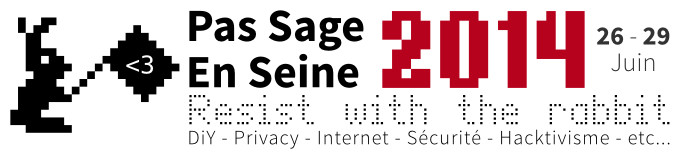
\includegraphics[scale=0.5] {logoPSES.jpg} 
\end{center}
\end{frame}


%----------------------------------------------------------------------------------------
\begin{frame}

\Huge{\centerline{Merci de votre attention.}}
\Huge{\centerline{Place aux questions. Débatons...}}

\begin{columns}[c] 
\column{.50\textwidth} 

\includegraphics[width=2.5cm,height=2.5cm]{./Genma.jpg} 
\column{.50\textwidth} 
\Large{
\begin{itemize}
\item Le Blog de Genma \\ http://genma.free.fr
\item Twitter @genma
\end{itemize}
}
\end{columns}

\end{frame}
\end{document}